\documentclass[11pt,a4paper]{article}

\usepackage[margin=1in]{geometry}
\usepackage{times}
\usepackage{graphicx}
\usepackage{booktabs}
\usepackage{hyperref}
\usepackage{amsmath,amssymb}
\usepackage{microtype}
\usepackage{xcolor}
\usepackage{caption}
\usepackage{subcaption}
\usepackage{enumitem}

\hypersetup{
  colorlinks=true,
  linkcolor=black,
  citecolor=blue!50!black,
  urlcolor=blue!50!black
}

\title{Mixture of Models:\\
Latency-Transparent Composition of Heterogeneous Predictors}
\author{Aquin Labs\\
\texttt{github.com/aquinlabs/mom}}
\date{}

\begin{document}
\maketitle

\begin{abstract}
Many deployed AI systems already combine multiple models---routers, small and large language models, captioners, classifiers---yet the composition layer is usually an ad hoc script that exposes seams: extra latency, tone flips, and visible routing.
We present \textbf{MoM} (\emph{Mixture of Models}), a colocated composition runtime whose call surface behaves like a single model.
Graphs are data: nodes name directory ids; edges are ordinary dependencies or \emph{speculate} edges that overlap a cheap router with a likely prior generator.
On a hit, wall time is approximately $\max(\text{router}, \text{prior})$; on a miss the prior is cancelled and the routed model runs.
A thin Python SDK wraps a Rust hot path for planning, shared state, and timing.
On a mixed text eval with SmolLM2-135M/360M, MoM matches always-strong accuracy while beating always-strong on easy latency and total wall time, with orchestration overhead on the order of $0.2\,\mathrm{ms}$.
Vision graphs that feed BLIP captions into MoM chat dominate torchvision ResNet18$\rightarrow$chat on the same synthetic pixel set, clarifying when a vision hop is a useful bus versus ImageNet cosplay.
\end{abstract}

\section{Introduction}
\label{sec:intro}

Production assistants rarely call one checkpoint.
They classify intent, retrieve, caption an image, then generate---often with a small model on easy turns and a larger one when the prompt is hard.
Frameworks for serving~\cite{kwon2023vllm} and decoding~\cite{leviathan2023speculative,chen2023accelerating} optimize \emph{inside} a model; sparsely gated MoE layers~\cite{shazeer2017moe,jiang2024mixtral} mix experts \emph{inside} one trained network.
What is missing is a first-class runtime for composing \emph{already trained}, modality-heterogeneous models so the \emph{external} experience matches one model: shared state, speculative routing, and orchestration cost that stays under natural model variance.

\textbf{MoM} is that runtime~\cite{mom2025}.
Its thesis is narrow and measurable: composition should feel seamless when the graph shape allows latency hiding, and should fail loudly (miss path) when it does not.
This paper describes the contracts, the speculate scheduler, and empirical results on text and vision graphs using real Hugging Face and torchvision~\cite{torchvision2016} weights---not stubs.

\paragraph{Contributions.}
\begin{itemize}[leftmargin=*]
  \item A thin \textbf{Model} contract and \textbf{ModelDirectory} so any adapter (chat, router, caption, classifier) registers by id.
  \item \textbf{Graphs as data} with \texttt{depend} and \texttt{speculate} edges, executed by a Rust-backed planner with cooperative cancel.
  \item A product SDK (\texttt{MoM()}, \texttt{Session}, CLI, HTTP) over the same hot path.
  \item Measurements: text speculate vs always-fast/always-strong; vision caption vs torchvision ResNet hops into the same chat stack.
\end{itemize}

\section{Related work}
\label{sec:related}

\textbf{Speculative decoding} drafts tokens with a small model and verifies with a large one~\cite{leviathan2023speculative,chen2023accelerating}.
MoM's speculate edge is coarser: it overlaps a \emph{router} with a prior \emph{full generation}, not draft tokens.
\textbf{Mixture-of-Experts} trains sparse experts inside one network~\cite{shazeer2017moe}.
MoM mixes independently trained models and tools.
\textbf{Serving stacks} (e.g.\ vLLM) maximize throughput for a model process~\cite{kwon2023vllm}; MoM sits above adapters and cares about inter-model wall time.
\textbf{Vision-language} systems such as BLIP~\cite{li2023blip} produce captions; ImageNet ResNets~\cite{he2016resnet} produce class scores.
We treat both as MoM hops and show they are not interchangeable buses into chat.

\section{System}
\label{sec:system}

\subsection{Contracts}
A \textbf{Model} implements \texttt{run(input, state, cancel=None) $\rightarrow$ output}.
There is no modality hierarchy: chat, routers, captioners, and torchvision classifiers share the method.
A \textbf{ModelDirectory} maps string ids to factories plus tags/metadata.
A \textbf{StateStore} is single-owner shared memory across hops and turns; models read/write keys instead of owning the message bus.
A \textbf{Graph} is a list of nodes (name, model id) and edges of kind \texttt{depend} or \texttt{speculate}.

\subsection{Speculative scheduling}
\begin{figure}[t]
  \centering
  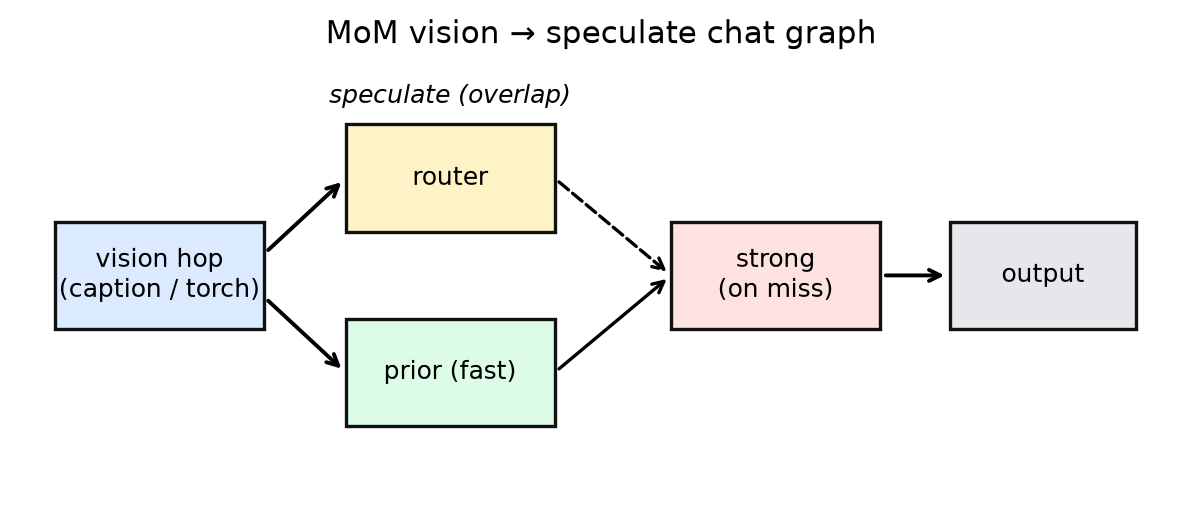
\includegraphics[width=0.95\linewidth]{figs/architecture.png}
  \caption{Vision hop into a speculate-chat graph. The router and prior (fast) start together; on a miss the prior is cancelled and the strong model runs.}
  \label{fig:arch}
\end{figure}

For edge $\texttt{speculate}(\textit{router}, \textit{prior})$, the scheduler starts both when the router becomes ready.
If the router's decision matches the prior's model id (\emph{hit}), wall time is approximately $\max(t_{\mathrm{router}}, t_{\mathrm{prior}})$ and the prior output is kept.
On a \emph{miss}, the prior receives a cancel token (best-effort) and the routed model runs; correctness is preserved, latency is not hidden.
Orchestration overhead is reported separately from model time; the design bar is that this overhead stay $\ll$ natural variance of the adapters.

\subsection{SDK surface}
\texttt{run(graph, input, directory)} returns output plus metrics (\texttt{total\_ms}, \texttt{orchestration\_overhead\_ms}, per-edge \texttt{spec}).
\texttt{Session} keeps one store across turns.
\texttt{MoM()} loads a production directory (local HF / path weights by default), a graph registry, and exposes \texttt{chat} / \texttt{run} / \texttt{serve}.
A CLI (\texttt{mom doctor|models|graphs|plan|run|chat|serve}) wraps the same handle.

\subsection{Production graphs}
Named graphs include \texttt{speculate\_chat}, \texttt{direct\_fast}, \texttt{direct\_strong}, and vision variants:
\texttt{caption\_chat} (BLIP$\rightarrow$router$\|$fast), \texttt{torch\_chat} (ResNet18$\rightarrow$router$\|$fast), and their always-strong baselines.
Figure~\ref{fig:arch} sketches the vision$\rightarrow$speculate shape.

\section{Experimental setup}
\label{sec:setup}

\paragraph{Text.}
Fast and strong generators are SmolLM2-135M and SmolLM2-360M Instruct~\cite{allal2025smollm2}.
A heuristic router chooses fast on short factual prompts and strong on hard ones.
Eval: 24 easy + 8 hard prompts, two rounds ($n{=}64$ per arm), comparing MoM \texttt{speculate\_chat}, always-fast, and always-strong.
Cost uses a proxy $\textit{work}=\sum \textit{tokens}\times\textit{params}_M$.

\paragraph{Vision.}
We use synthetic PNGs (solid colors, circle, split red/blue) so ground truth is unambiguous (Figure~\ref{fig:montage}).
Caption hop: BLIP base~\cite{li2023blip}.
Torch hop: torchvision ResNet18~\cite{he2016resnet,torchvision2016} with ImageNet logits written into state for the chat hop.
Graphs: \texttt{caption\_chat}, \texttt{caption\_strong}, \texttt{torch\_chat}, \texttt{torch\_strong}.

\begin{figure}[t]
  \centering
  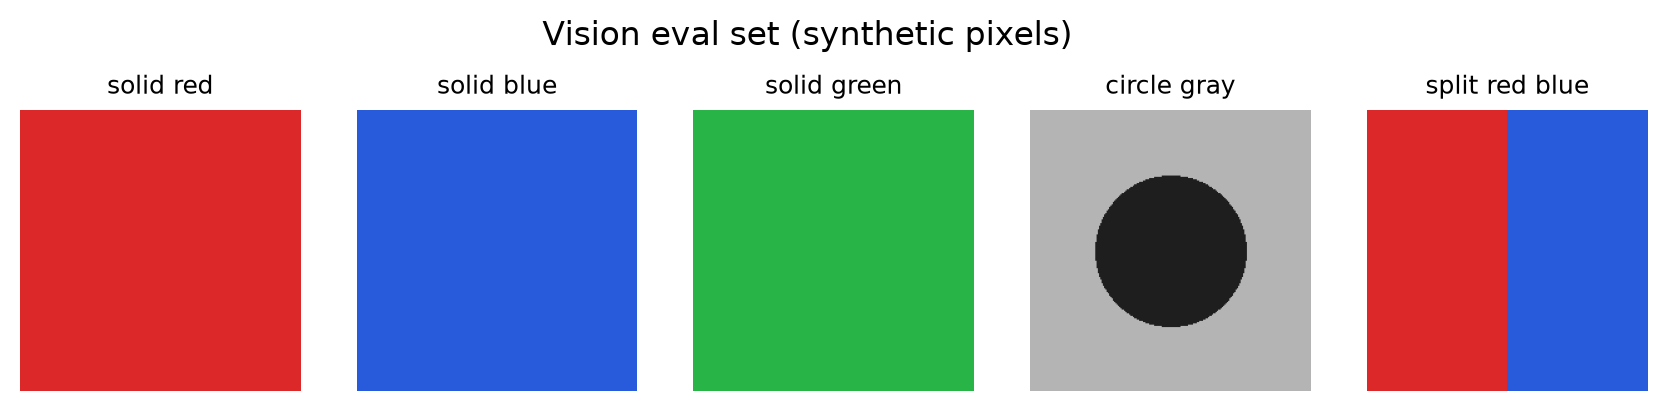
\includegraphics[width=0.95\linewidth]{figs/eval_montage.png}
  \caption{Synthetic vision eval images used by the MoM vision proof.}
  \label{fig:montage}
\end{figure}

\section{Results}
\label{sec:results}

\subsection{Text: MoM vs always-fast / always-strong}
\begin{figure}[t]
  \centering
  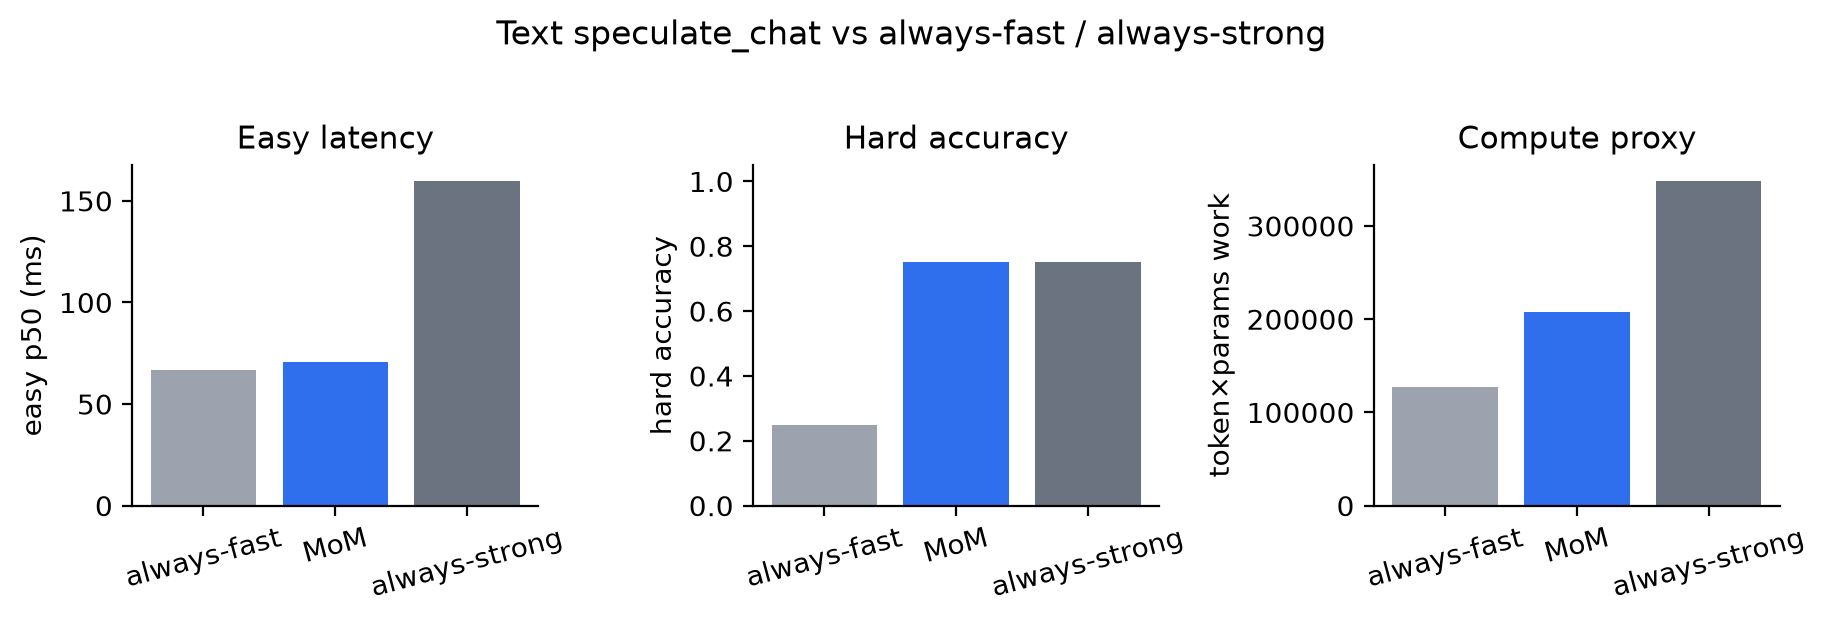
\includegraphics[width=0.98\linewidth]{figs/text_scoreboard.png}
  \caption{Text scoreboard from \texttt{mom\_proof} / \texttt{mom\_cost}: MoM matches always-strong hard accuracy, cuts easy p50 roughly in half vs always-strong, and uses $\sim$0.60$\times$ the token$\times$params work of always-strong.}
  \label{fig:text}
\end{figure}

Table~\ref{tab:text} and Figure~\ref{fig:text} summarize the text bakeoff.
MoM easy p50 is $70.6\,\mathrm{ms}$ vs $159.6\,\mathrm{ms}$ for always-strong, with $48/48$ easy hits onto fast.
Hard accuracy matches always-strong at $75\%$ (always-fast collapses to $25\%$), with $16/16$ intentional misses.
Total wall on the mixed set: MoM $11.5\,\mathrm{s}$ vs always-strong $17.1\,\mathrm{s}$.
Orchestration p50 is $0.17\,\mathrm{ms}$.
Compute proxy: MoM work is $0.60\times$ always-strong.

\begin{table}[t]
\centering
\caption{Text speculate\_chat vs single-model baselines ($n{=}64$).}
\label{tab:text}
\begin{tabular}{lcccc}
\toprule
Arm & Acc & Easy p50 & Hard acc & Orch p50 \\
\midrule
always-fast   & 81.3\% & 66.7\,ms & 25\% & $<$0.02\,ms \\
\textbf{MoM}  & \textbf{93.8\%} & \textbf{70.6\,ms} & \textbf{75\%} & 0.17\,ms \\
always-strong & 93.8\% & 159.6\,ms & 75\% & $<$0.02\,ms \\
\bottomrule
\end{tabular}
\end{table}

\subsection{Vision: caption bus vs torchvision bus}
\begin{figure}[t]
  \centering
  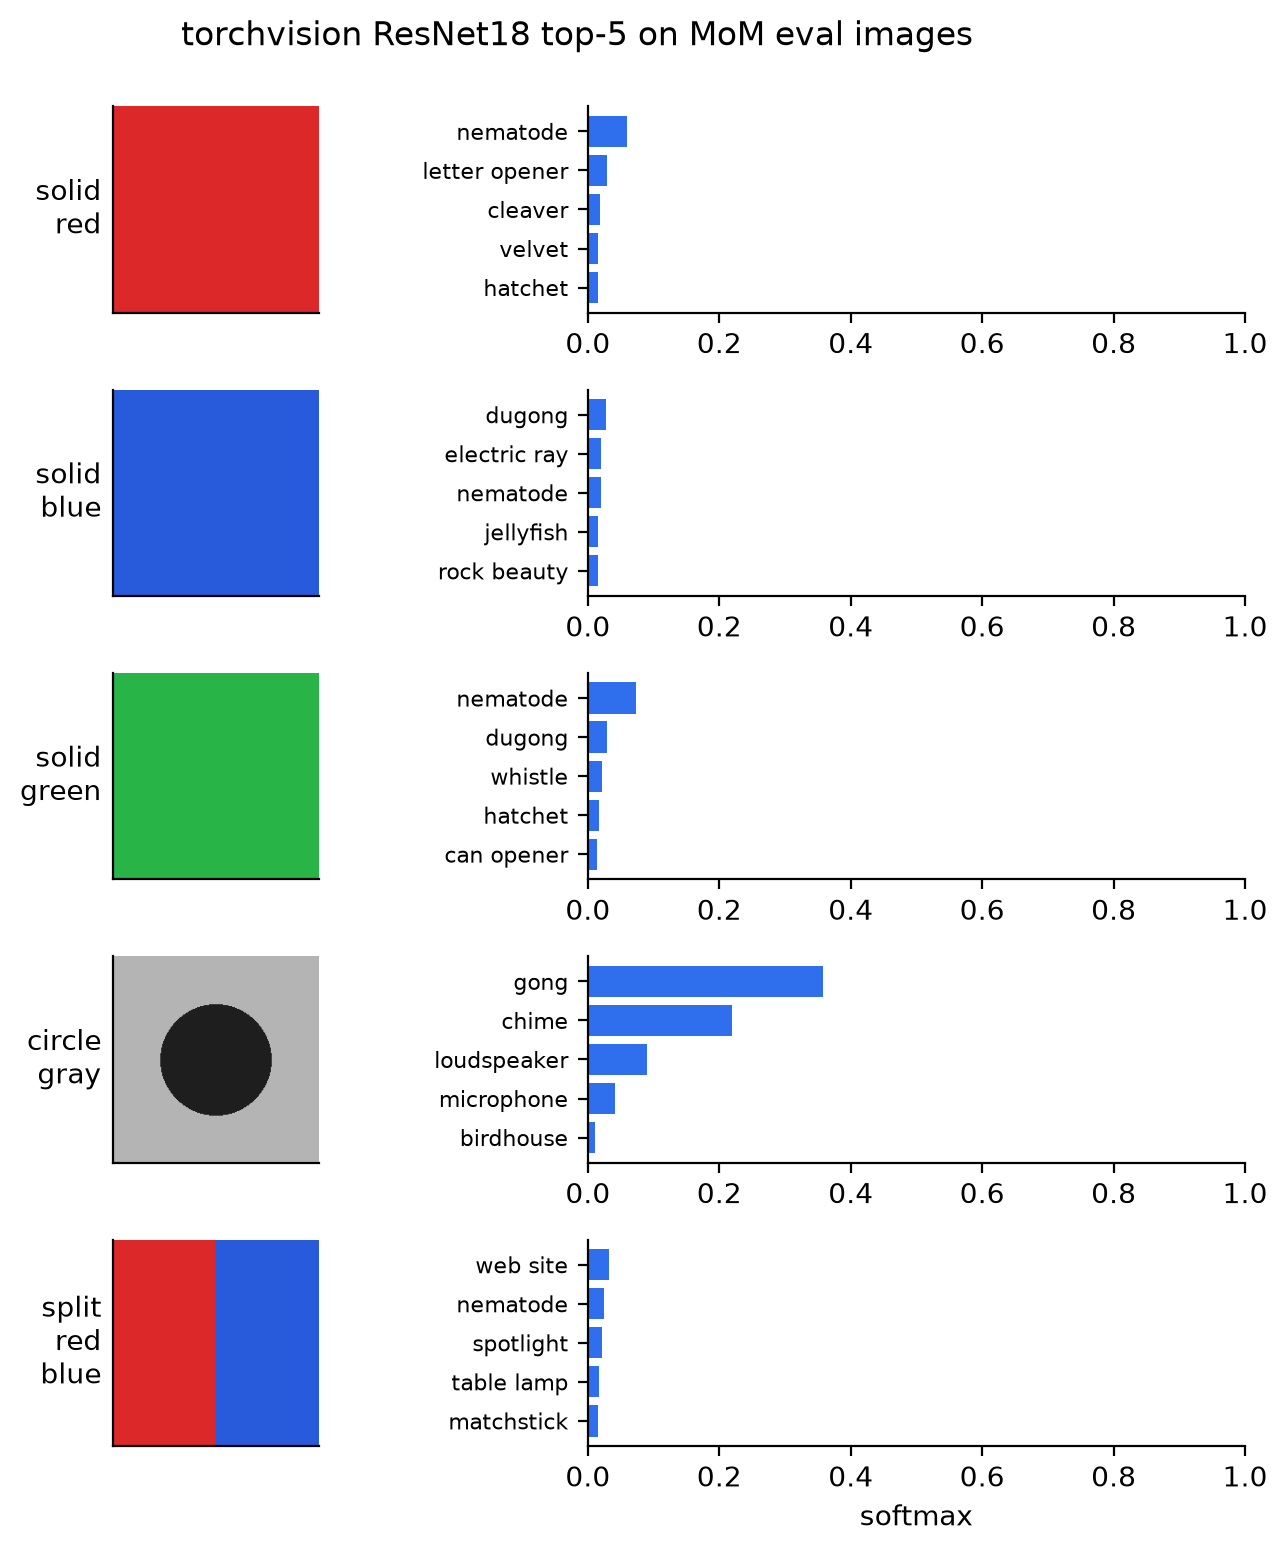
\includegraphics[width=0.98\linewidth]{figs/torch_topk.png}
  \caption{ImageNet top-5 from torchvision ResNet18 on the MoM eval set. Solid colors and simple shapes are not ImageNet concepts; the classifier is the wrong semantic bus for color/shape QA.}
  \label{fig:topk}
\end{figure}

\begin{figure}[t]
  \centering
  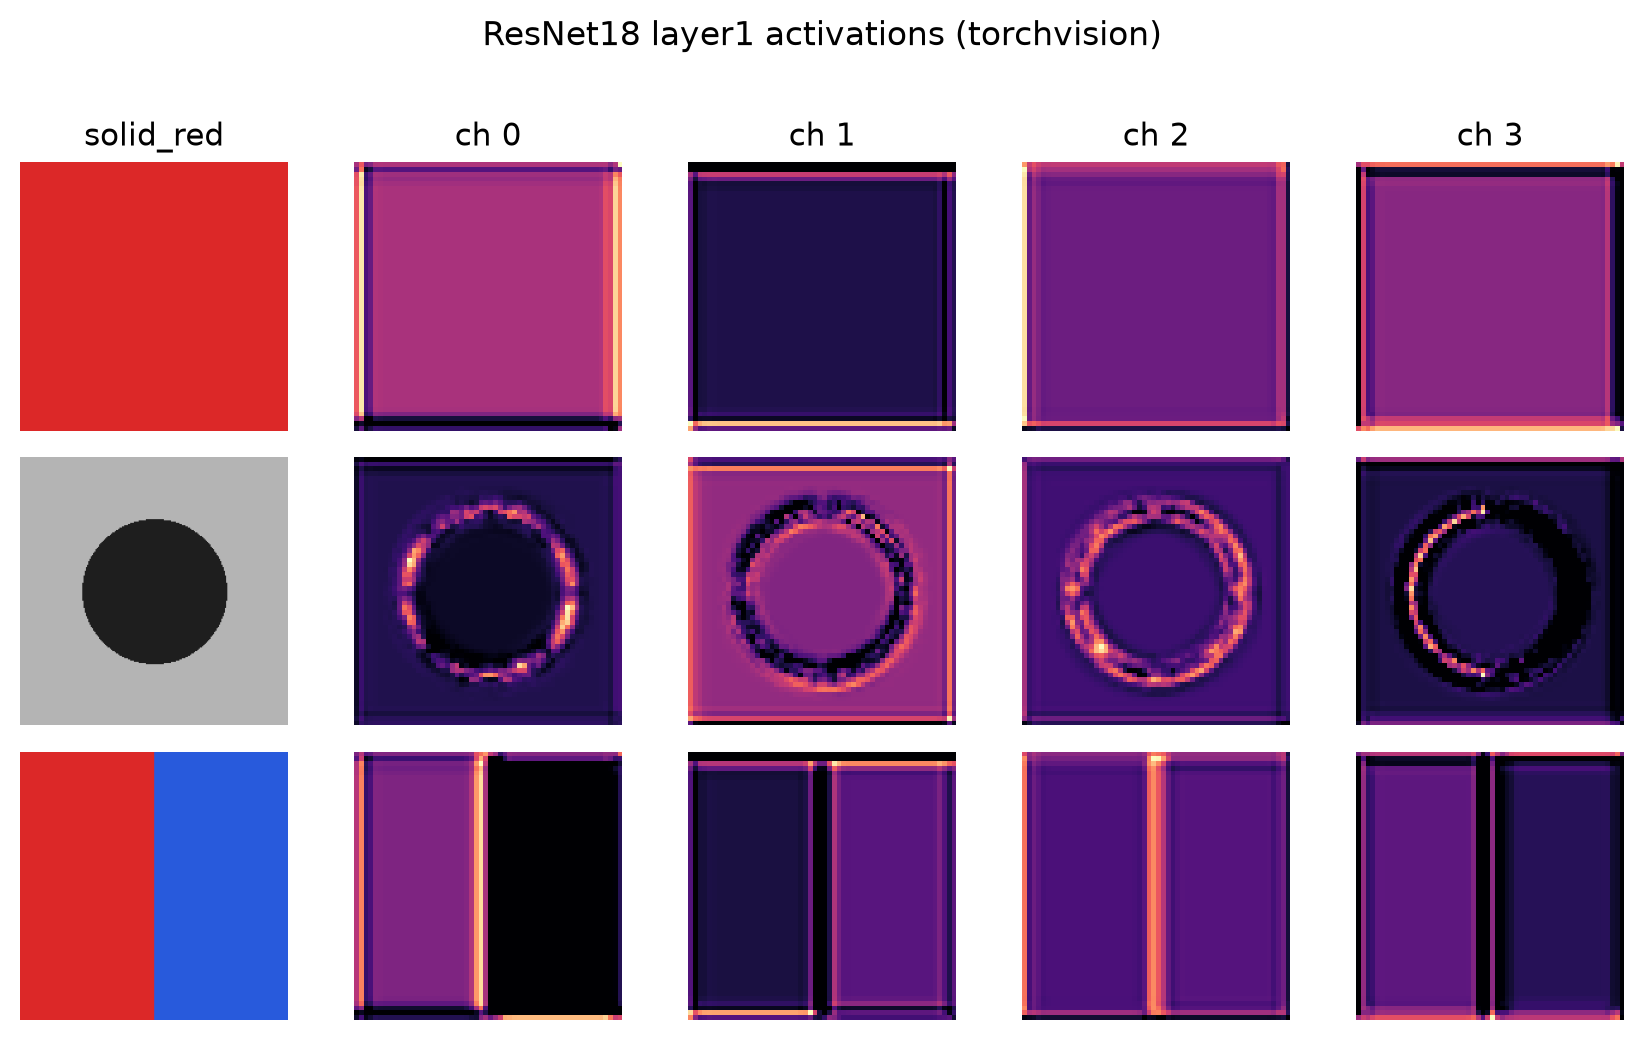
\includegraphics[width=0.98\linewidth]{figs/torch_activations.png}
  \caption{ResNet18 \texttt{layer1} channel activations on three eval images (torchvision weights). Early maps respond to coarse structure; they do not recover ``red'' / ``blue'' as chat-ready language.}
  \label{fig:acts}
\end{figure}

Figure~\ref{fig:topk} shows ResNet18's ImageNet top-5 on each eval image: solid red/blue/green do not land on color words, so a chat hop conditioned on those labels is poorly grounded.
Figure~\ref{fig:acts} visualizes early activations---useful as a systems figure, not as a VQA answer.

\begin{figure}[t]
  \centering
  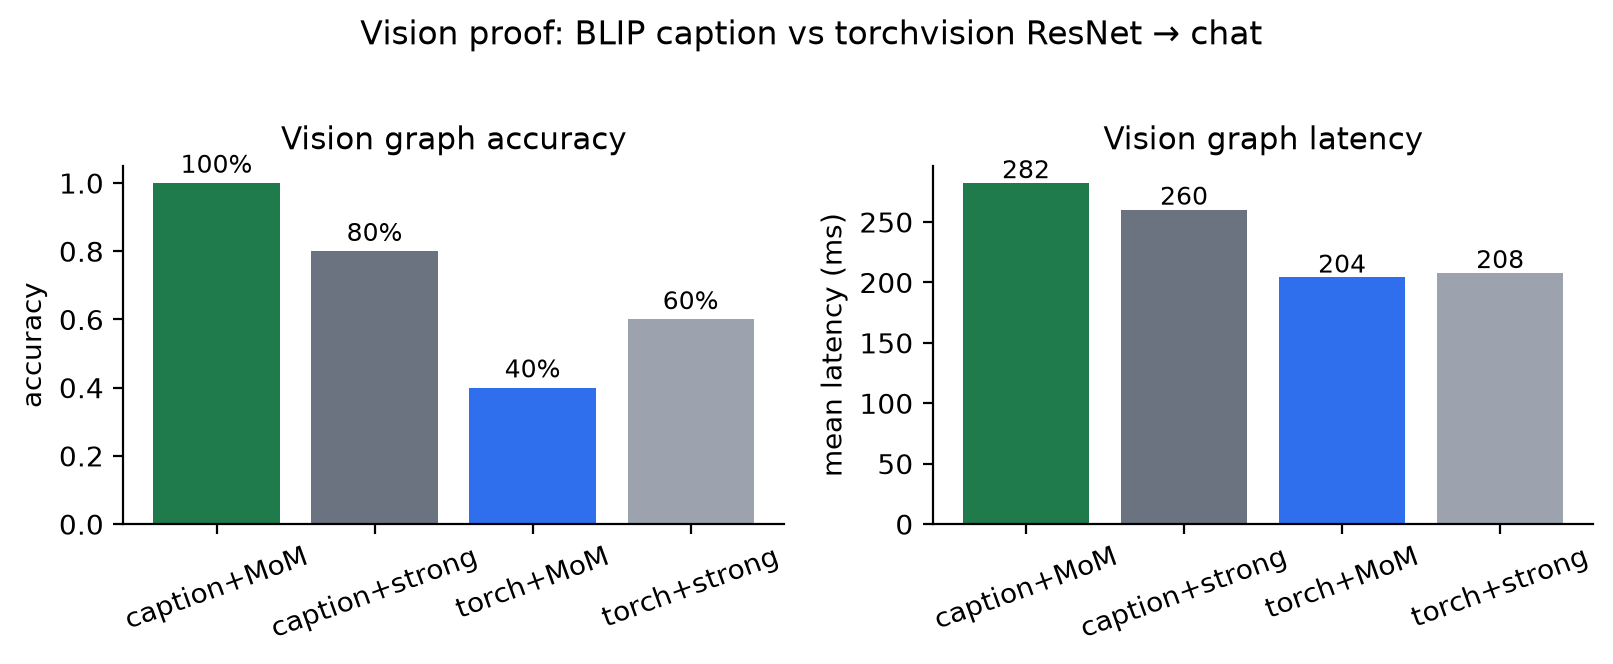
\includegraphics[width=0.98\linewidth]{figs/vision_scoreboard.png}
  \caption{Vision graph accuracy and mean latency. Caption$\rightarrow$MoM reaches $100\%$ on this set; torch$\rightarrow$MoM drops to $40\%$.}
  \label{fig:vision}
\end{figure}

\begin{figure}[t]
  \centering
  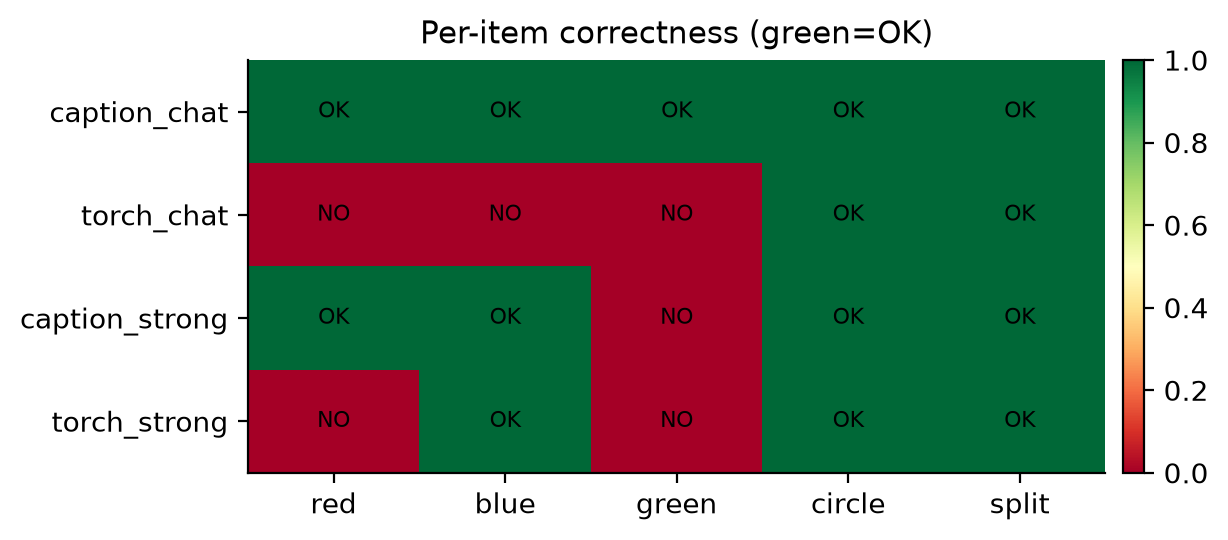
\includegraphics[width=0.85\linewidth]{figs/vision_per_item.png}
  \caption{Per-item correctness across vision arms. Caption graphs succeed on color questions where torch graphs fail.}
  \label{fig:peritem}
\end{figure}

On the five-image set (Figure~\ref{fig:vision}, Table~\ref{tab:vision}), \texttt{caption\_chat} is $5/5$ correct; \texttt{torch\_chat} is $2/5$.
Always-strong variants do not rescue the torch bus: the failure is the vision representation, not the generator size.
This is the intended lesson: MoM will compose whatever you register; useful MoM is \emph{tools + right bus + speculate}, not classifier cosplay.

\begin{table}[t]
\centering
\caption{Vision proof tallies (5 images). Mean latency in ms.}
\label{tab:vision}
\begin{tabular}{lcc}
\toprule
Arm & Acc & Mean ms \\
\midrule
caption\_chat   & 100\% & 282 \\
caption\_strong & 80\%  & 260 \\
torch\_chat     & 40\%  & 204 \\
torch\_strong   & 60\%  & 208 \\
\bottomrule
\end{tabular}
\end{table}

\section{Discussion}
\label{sec:discussion}

\paragraph{What speculate can hide.}
Hit paths hide router cost under the prior.
Miss paths are correct and visible---that is a feature for measurement and for users who need the strong model.
Serial pipelines and heavy reconcile after fan-out are valid graphs; they are not latency-hideable~\cite{mom2025}.

\paragraph{Cost vs speed.}
When always-strong is the accuracy bar, MoM's win is often cheaper work (token$\times$params) and lower mixed-set wall time, not a claim that every hit is faster than a tiny model alone.

\paragraph{Limits.}
v1 is colocated; shared state is not multi-host.
Cancel is cooperative.
Vision results use a tiny synthetic set to isolate bus quality; they are not a general VQA benchmark.
We do not claim bit-identical outputs across model versions.

\section{Conclusion}
\label{sec:conclusion}

MoM makes heterogeneous model composition a runtime concern: register adapters, wire graphs, call one surface.
With speculative routing, orchestration stays negligible while easy turns stay on a small LM and hard turns reach a larger one.
Vision graphs reinforce that the hop you wire matters as much as the scheduler: BLIP captions compose; ImageNet ResNet scores on solid colors do not.
The open-source SDK, CLI, and harnesses are the reproducible artifact~\cite{mom2025}.

\section*{Acknowledgments}
Built at Aquin Labs. Measurements used local HF and torchvision weights via the MoM production directory.

\bibliographystyle{plain}
\bibliography{refs}

\end{document}
